\begin{figure*}[t]
    \centering
    \begin{minipage}{0.49\textwidth}
        \centering
        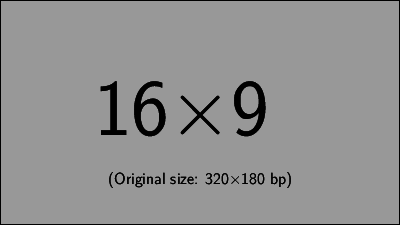
\includegraphics[width=\textwidth]{assets/mwe/example-image-16x9}
        \caption{Local Temporal Modeling}
        \label{figure:local-temporal-modeling}
    \end{minipage}
    \hfill
    \begin{minipage}{0.49\textwidth}
        \centering
        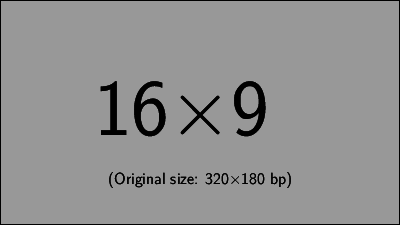
\includegraphics[width=\textwidth]{assets/mwe/example-image-16x9}
        \caption{Global Temporal Modeling}
        \label{figure:global-temporal-modeling}
    \end{minipage}
\end{figure*}

\section{Our Approach}

Given the dataset size constraint we are faced with, it is obvious that training a neural network from scratch only with our data is completely infeasible and wouldn't yield any results.

This is why we took the decision to profit from networks that are pre-trained on popular huge datasets that ressembles the kind of actions available in ours and thus profit and take advantage of the features learned by this networks. In simple words the idea is to take pre trained networks and extract the representation they make of our videos, clips, frames in their hidden layers and use it for classification by passing it into another network we would make.
The idea is that this network we are going to use as a backbone for sure contains some relevant features that understand the video teporality and sptiality in some way and this features must contains enough information about the video segment to do some sort of classification such as for the kinetics dataset, and thus we'll try to extract this information and use it in order to classify on our custom classes. 

In addition to minimizing the damage made by the dataset constraints, taking this approach also reduces the required computational power as it is limited in our case, since we are not training a big network from scratch. And on top of that designing a neural network architecture would require more expertise and time (only 120 hours for the research project) which i don't have yet.

\begin{figure*}[t]
    \centering
    \begin{minipage}{0.49\textwidth}
        \centering
        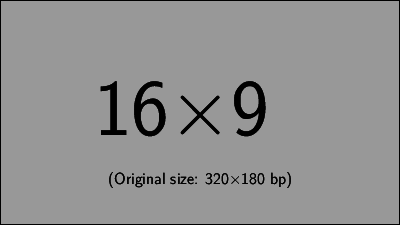
\includegraphics[width=\textwidth]{assets/mwe/example-image-16x9}
        \caption{Illustration of our Model}
        \label{figure:local-temporal-modeling}
    \end{minipage}
\end{figure*}

\subsection*{Considered Variants}

As the temporal context window of the backbone networks is quite limited to around 16-32 frames usually, processing the whole 4 mins of video and extracting a single feature for the whole video is both computationally costly and not practical in our case (would be practical for video classification) since we want to extract the different time segments and classify them rather than classifying the whole video.
This is why we present two approaches.

\subsection{Local Temporal Modeling}
It is called like that as we take a video segment of N frames (N depend on the backbone model being used), extract the features from it and use this features to perform classification.
This method is quite straightforward and easy to implement but the main issue is that we are ignoring the fact that the small video segments belong to the same video, as the classification model 
can maybe benefit from that and maybe some actions only happen at certain moments of the climb, this can also reduce and prevent the noise in classes as the model wouldn persist a class in time rather than keeping it only for 32 frames.

\todo[inline]{Talk about positional embedding.}
\todo[inline]{Reference the figure.}

\subsection{Global Temporal Modeling}

\todo[inline]{Talk about the possible use of attention in this case and how it affects the performance, maybe it allows the model to only focus on the last frames which is the most important ?}

In order to achieve that we are going to use an LSTM for the classification network rather than an MLP. We keep the LSTM very simple and lightweight with only a single layer just like the MLP in order to avoid overfiting given our dataset size.

\todo[inline]{Reference the figure.}

\subsection*{Feature Extractors}
Multiple options are available for the backbone model that will perform feature extractions, we can distinguish two types: Frame Level Feature Extractor and Segment / Video Level Feature Extractor.

\todo[inline]{Talk about temporal sub sampling and justify it's use by the dears of the papers in the field that says it is very efficient and that it reduces computations a lot and that it is trivial and logique to think that it won't drop performance as there isn't a lot of change betwen two consecutive frames.}

\textbf{Frame Level Feature Extractor}
This can essentially be any model that extract some features given a frame, it can be a 2D CNN model such as 2D ResNet, etc, a Vision Transformer such as Deno, Clip, Google ViT, etc or some custom handmade features such as using Yolo keypoints or positions or presente of certain objects such as a brush, elevation of the climber, etc.

This type of feature extractor is very convenient as pre-trained image feature extractors are very abundant as many years have passed through the subject and enough time for it to murir.

Extracting custom features can be tricky and hard to do, for example we could check whether a brush is present on the frame or not and if it is close to the climber, while this is a good idea the thing is that the brush can take different forms in different climbing competition and isn't necesarily a brush, on top of that this requires training a networ for object detection which is costy both in data and computation which are two things we don't have.

Thus we'll mainly stick to the automatic feature extractors during this study.

A question arise from  the frame level feature extractors which is how to combine the frames features into a single feature representing the clip / segment of the video from which the frames have been taken ?

We can distinguish three main possibilities:

The first one is to concatenate the different features forming a single big one, this is the easiest method but not convinient at all as it can form big vectors that don't necessarily have sense.

The second one would be to average (or add them) the different features of the frames and come up with a single one. Doing that for the YOLO model would be just like taking the average position of the climber during the video segment.
\todo[inline]{Cite that in the deno paper and lot of other ones, it is recommanded that taking the average works well.}

The third one which is the most interesting would be to temporally model (link them) this features using an LSTM (in order to create the temporal dependence and come up with a feature that is temporally aware) in order to come up with a single feature representing the video. This approach is certenly the most interesting one.

The cons of temporal modeling is the introduction of another component into the architecture which complexify it and add parameters.

We could also use some linear layer in order to combine them.

\todo[inline]{Here we'll briefely describe the feature extractors we used and more importantly their types (Frame level, Segment level, Slow fast, etc. The goal isn't to fully detail them as this will be done in the )}

\textbf{Video / Clip / Segment Level Feature Extractor}

This models are usually 3D CNNs that have been created and trained by inflating 2D CNNs with some additional things. More recently Transformers have been employed for this and are working pretty well but the issue with that is the rquireemnt of huge computational power and datasets to compensate the lack of inductive baies which is present in CNNs for example.

Using this type of feature extractor, no further processing is required to be done on the videos.

\subsection{Training - Methodology}

\todo[inline]{Talk about how we setup training}
\todo[inline]{Talk about data filtering and what we have done to improve the results such as removing personless and multi person frames, getting rid of low quality data such as unanotatated rather than puting a nothing label, etc}
\todo[inline]{Talk about the training setup that was used.}